% !TEX encoding = UTF-8 Unicode
\documentclass{report}
%\usepackage{xeCJK}

%\setCJKmainfont{微软雅黑}
\title{test Collection}
\author{Michael Jordan}
\date{\today}
	
% big font for sections
\usepackage{sectsty}
\usepackage{setspace}
\sectionfont{\LARGE}

\usepackage{graphicx}
\usepackage{wrapfig}
\usepackage{caption}
\usepackage{subcaption}
\usepackage{listings}
\usepackage{array}
\usepackage{titlesec}
\setcounter{secnumdepth}{5}
\usepackage[colorlinks,
linkcolor=black,
anchorcolor=black,
citecolor=black
]{hyperref}
\lstset{
    columns=fixed,       
    numbers=left,                                        % 在左侧显示行号
    frame=none,                                          % 不显示背景边框
    backgroundcolor=\color[RGB]{245,245,244},            % 设定背景颜色
    keywordstyle=\color[RGB]{40,40,255},                 % 设定关键字颜色
    numberstyle=\footnotesize\color[RGB]{0,0,0},           % 设定行号格式
    commentstyle=\it\color[RGB]{0,96,96},                % 设置代码注释的格式
    stringstyle=\rmfamily\slshape\color[RGB]{128,0,0},   % 设置字符串格式
    showstringspaces=false,                              % 不显示字符串中的空格
    language=c++,                                        % 设置语言
    morekeywords={alignas,continute,friend,register,true,alignof,decltype,goto,
    reinterpret_cast,try,asm,defult,if,return,typedef,auto,delete,inline,short,
    typeid,bool,do,int,signed,typename,break,double,long,sizeof,union,case,
    dynamic_cast,mutable,static,unsigned,catch,else,namespace,static_assert,using,
    char,enum,new,static_cast,virtual,char16_t,char32_t,explict,noexcept,struct,
    void,export,nullptr,switch,volatile,class,extern,operator,template,wchar_t,
    const,false,private,this,while,constexpr,float,protected,thread_local,
    const_cast,for,public,throw,std},
}

% \begin{comment} ... \end{comment{}
%\usepackage{verbatim}

\setlength{\parskip}{0pt}

\makeatletter
\renewcommand{\paragraph}{
  \@startsection{paragraph}{4}
    {\z@}{1.25ex \@plus 1ex \@minus .2ex}{-1em}
      {\normalfont\normalsize\bfseries}
      }
      \makeatother

\usepackage[
	sorting=none,
	minbibnames=8,
	maxbibnames=9,
	block=space,
	backend=biber
]{biblatex}
\bibliography{publications}


\usepackage{parskip}

\usepackage{lipsum}

\begin{document}

\newpage

\maketitle

\newpage

\renewcommand{\contentsname}{Table of Content}
\tableofcontents


%=================
\begin{spacing}{1.5}

\section{Overview}

\subsection{问题描述}

\begin{itemize}

\item{\Large{编写一个函数,计算逻辑表达式的真值表}}
	\begin{itemize}
		\item	逻辑表达式最多有8个输入项,分别为$A,B,C,D,E,F,G,H$;

		\item	支持的逻辑运算符按优先级从高到低分别为$\sim$(非)、$\&$(与)、$\land$(异或)、$\mid$(或);
	
	\end{itemize}
\item{\Large{编写一个函数,根据真值表计算逻辑表达式,以字符串格式输出}}
	\begin{itemize}
		\item	使用Quine-McCluskey算法对逻辑表达式进行化简。	
	\end{itemize}

\item{\Large{函数接口:}}
	\begin{itemize}
		\item	std::string expr$\_$to$\_$truthtable(int n, const std::string$\&$ expr);

其中n是变量个数,expr是逻辑表达式,返回真值表。

		\item	std::string truthtable$\_$to$\_$expr(const std::string$\&$ truth$\_$table);

其中truth$\_$table是真值表,返回逻辑表达式。
	
	\end{itemize}

若参数无效,函数抛出异常。

\item{\Large{要求}}
	\begin{itemize}
		\item	使用第5讲的测试框架对两个函数进行测试;提交源代码与设计文档。
		\item	文档内容包括:设计思路、数据结构与算法、重要的类与函数的说明、测试用例的设计等等,也可以写完成Project的心得体会、经验与教训等。
	
	\end{itemize}

\end{itemize}

\subsection{解题概况}
	最终程序各部分及其作用如下表

	\begin{center}
		\begin{tabular}{|c|c|}
			\hline  Documents & Functions\\
			\hline  constants.h & 常量的定义\\
			\hline  simple$\_$test.h & 参与测试\\
			\hline  ChartToExpression.h & 将真值表转换为逻辑表达式\\
			\hline  ExpressionToChart.h & 将逻辑表达式转换为真值表\\
			\hline  implication & 质蕴涵项的实现\\
			\hline
		\end{tabular}
	\end{center}	
	
	下面就各部分的解题思路及实现进行详细讨论	
\section{主要思路}

本次Project分为两部分,下面就这两部分分别进行讨论:

\subsection{expr$\_$to$\_$truthtable}
	首先,通过将题目抽象,这一部分是一个经典的表达式求值的问题,其主要问题如下:
		$$\mbox{利用算符优先关系,实现对给定混合运算表达式的求值。}$$
		
	这是个栈的经典应用问题,常见解法是将中缀表达式(即输入的表达式)转化为后缀表达式后求解。时间复杂度为$O(n)$,其中$n$为变量的个数
	
	具体的算法会在main$\_$algorithm模块详细介绍。
	
	表达式求值是一个非常经典的问题,已经有了许多成熟的解法。甚至在Python中,一条evaluate语句就可以完成这样的工作。但是对于含字母的表达式,至今没有太好的解决办法。
	
	但是考虑到本次作业的特殊性,一共只有最多8个变量,同时是逻辑计算而不是算术计算,这无疑极大的降低了难度。对于普通的算术含参表达式,我们只能多次取不同的大素数代入变量,还不能保证正确性。但是在本题的布尔代数式中,一共只有$2 ^ 8 = 256$种取值方式,是完全可以接受的。于是,我们可以先遍历所有变量的可能取值,代入表达式中,从而计算出真值表中对应的值。
	
	因此,总的时间复杂度为$O(n * 2 ^ n)$, 由于 $n \le 8$,复杂度不会超过$8 * 2 ^ 8 = 2048$,是完全可以接受的。
\subsection{truthtable$\_$to$\_$expr}

	对于将真值表转化为表达式的问题,我们在数字逻辑电路中曾学习过使用卡诺图的方法,非常直观,同时在对于维数较低时也易于化简。
	
	但是卡诺图的解题过程较为繁琐,同时对于高维的情况扩展性较差。在$n \geq 6$时,就比较难画出合适的卡诺图了。因此,我们选用Quine-McCluskey算法。它虽然较为抽象,但是非常模式化,对高维的扩展性很好。
	
	至于算法的时间复杂度方面,由于化简表达式至今还是NP-hard问题,因此只存在指数级解法,即问题的时间复杂度为$O(2 ^ n)$
	
	同时,题目要求将表达式化到最简形式,因此在Quine-McCluskey算法后我们必须进行化简。这里采用petrick化简算法,时间复杂度同样为$O(2 ^ n)$
	
	具体的算法会在main$\_$algorithm模块详细介绍。

\subsection{异常处理}
	我还没做呢
\section{Project Structures}
\subsection{ChartToExpression}

对于第一个问题,我们使用ChartToExpression类来实现,程序声明如下:

\lstinputlisting{sources/ExpressionToChart.txt}

其中各变量及函数作用如下:

\begin{itemize}
	\item{变量}
	\begin{center}
		\begin{tabular}{cc}
			变量 & 作用 \\
			operators[] & 储存定义的四种运算符\\
			Stack$\_$Operator & 运算符的堆栈 \\
			Stack$\_$Number & 运算结果的堆栈 \\
			loc[MAX$\_$N] & 储存字符出现位置,便于代入数值\\
		\end{tabular}
	\end{center}
	\item{函数}
	\begin{center}
		\begin{tabular}{cc}
			函数 & 作用 \\
			ExpressionToChart() & 构造函数\\
			virtual ~ExpressionToChart() & 析构函数 \\
			Stack$\_$Number & 运算结果的堆栈 \\
			string solve(int n, const string $\&$InString) & 
			\textbf{将输入的表达式转换为真值表输出}\\
			string filter(const string $\&$s) &
			将输入的表达式去除多余空格\\
			string InfixToPostfix(const string $\&$infix) &
			\textbf{中缀表达式转换为波兰式}\\
			void PushString(string $\&$s, const char $\&$ch) &
			转化时向波兰式中添加字符\\
			bool IsOperator(char ch) &
			判断当前字符是否为运算符\\
			int priority(char Operator) &
			若是运算符,返回其优先级 \\
			int SolvePostfix(const string $\&$postfix) &
			\textbf{计算后缀表达式的值}\\
			void GetTwoNumbers(bool $\&$first, bool $\&$second) &
			在运算结果栈中取出两个元素用于计算\\
			bool CalcEq(bool first, bool second, char op) &
			给定运算数和运算符,计算结果\\
		\end{tabular}
	\end{center}
\end{itemize}
\subsection{ExpressionToChart}
对于将真值表转换为表达式的问题,我们采用Quine-McCluskey算法,主要使用ExpressionToChart类实现。

同时,由于对质蕴涵项这一概念使用较多,因此将它单独建立implication类,以增强内聚度

implication类声明如下:
\lstinputlisting{sources/implication.txt}

其中各变量及函数作用如下:

\begin{itemize}
	\item{变量}
	\begin{center}
		\begin{tabular}{cc}
			变量 & 作用 \\
			int TotalVariables & 总变量个数\\
			int bit & 当前质蕴涵的二进制表示\\
			int xterm & 质蕴涵的任意项,该位为1即为任意项 \\
			int ones & 质蕴涵中1的个数 \\
			string exp & 当前质蕴涵的二进制表示(输出用)\\
			bool used & 表示该蕴涵项是否被覆盖(Q-M算法中)\\
			bool selected & 表示该蕴含项是否是出现在结果中(petrick化简) \\
			vector<int> ImpContained & 该质蕴涵包含的蕴涵项\\

		\end{tabular}
	\end{center}
	\item{函数}
	\begin{center}
		\begin{tabular}{cc}
			函数 & 作用 \\
			implication() & 默认构造函数\\
			virtual ~implication() & 析构函数 \\
			implication(int mask, int xterm, int TotalVariables) & 构造函数\\
			int CountOne(int x) & 统计x的二进制表示中1的个数\\
			string show(); & 输出该蕴涵项\\
		\end{tabular}
	\end{center}
\end{itemize}


ChartToExpression类声明如下:
\lstinputlisting{sources/ChartToExpression.txt}

其中各变量及函数作用如下:

\begin{itemize}
	\item{变量}
	\begin{center}
		\begin{tabular}{cc}
			变量 & 作用 \\
			int TotalVariables & 总变量个数 \\
			vector<int> MinTerm & 输入的最小项,用int表示\\
			vector<implication> imp & 储存最小项,参与Q-M算法计算\\
			vector<implication> roller & Q-M算法中与imp迭代的数组\\
			vector<int> MinTermCovered[1 << MAX$\_$N] &
			可以覆盖该最小项的所有蕴涵\\
			bool table[1 << MAX$\_$N][1 << MAX$\_$N] &
			可视化蕴涵与最小项的关系\\
			bool contained[1 << MAX$\_$N] & 
			表示每个蕴涵项是否需要petrick化简\\
			vector<implication> primes &
			储存质蕴涵项\\

		\end{tabular}
	\end{center}
	\item{函数}
	\begin{center}
		\begin{tabular}{cc}
			函数 & 作用 \\
			ChartToExpression() & 构造函数\\
			virtual ~ChartToExpression() & 析构函数\\
			string solve(const string $\&$truth$\_$table) &
			输入真值表,返回化简后表达式\\
			void Quine-McCluskey() & 实现Quine-McCluskey算法\\
			void Simplify() & 对结果化简,使用到了petrick算法\\
			int CountOne(int x) & 统计x的二进制表示中1的个数\\
			bool CheckContained(const implication $\&$imp, const int $\&$x) &
			判断蕴涵Imp是否包含了最小项x\\
			void ShowTable() & 将中间结果可视化\\
		\end{tabular}
	\end{center}
\end{itemize}


\section{Main Algorithm}

\subsection{ChartToExpression}
\subsubsection{遍历所有输入}
	首先,我们需要将含字母的表达式转换为只含有数字的表达式,以便后续计算。
	
	核心代码如下:
	\lstinputlisting{sources/algo_part0.txt}
	\begin{itemize}
		\item	首先,遍历输入的字符串,对于每一个字母,用$loc[]$数组记下它出现的位置
		\item	然后,我们使用变量$mask$来遍历$2 ^ n$种可能输入。由于输出格式的要求,我们采用倒序遍历,即从$2^n - 1$开始,到$0$结束。当$mask$值一定时,对于每一位$i$,可以用位运算$value = (mask >> i) \& 1$来得到第$i$个变量的值$value$。
		\item	得到第$i$个变量的值$value$之后,通过遍历$loc[i]$数组,就可以得到该变量所有出现的位置,从而进行替换。
		\item	由于变量只有$A - H$,取值也只有$0 - 1$,都只有一位,所以直接赋值即可。于是完成了从含字母表达式到纯数字表达式的转换。
	\end{itemize}
\subsubsection{表达式求值}
\paragraph{中缀转后缀\\}
	\subparagraph{中缀表达式与后缀表达式}
		\begin{itemize}
			\item{中缀表达式\\} 
			中缀表示法是算术表达式的常规表示法。称它为中缀表示法是因为每个操作符都位于其操作数的中间,这种表示法只适用于操作符恰好对应两个操作数的时候(在操作符是二元操作符如加、减、乘、除以及取模的情况下)。

			Syntax: operand1 operator operand2
			
			Example: (A+B)*C-D/(E+F)
			
			\item{后缀表达式\\}
			在后缀表示法中,操作符严格位于操作数后面。因其使表达式求值变得轻松,所以被普遍使用。

			Syntax  : operand1 operand2 operator
			
			Example : AB+C*DEF+/-
			\item	由于中缀表示法是书写表达式的常见方式,而后缀表达式更便于计算表达式的值,因此我们常常采用将中缀表达式转化为后缀表达式再求值的方法。
		\end{itemize}
	\subparagraph{具体算法\\}
	中缀转换为后缀的难点在于操作符的优先级处理。由于后缀的操作符紧跟在操作数后,我们可以用一个栈来存储操作符,具体流程如下:
	\begin{itemize}
		\item	初始化一个空堆栈,将结果字符串变量置空。
		\item	从左到右读入中缀表达式,每次一个字符。
		\item	如果字符是操作数,将它添加到结果字符串。
		\item	如果字符是个操作符,弹出操作符,直至遇见左括号、优先级较低的操作符或者同一优先级的右结合符号。把这个操作符压入堆栈。
		\item	如果字符是个左括号,把它压入堆栈。
		\item	如果字符是个右括号,在遇见开括号前,弹出所有操作符,然后把它们添加到结果字符串。
		
		\item	如果到达输入字符串的末尾,弹出所有操作符并添加到结果字符串。
	
	\end{itemize}
	
	Project中,用$InfixToPostfix$函数实现:
	\lstinputlisting{sources/algo_part1.txt}	
\paragraph{后缀表达式求值\\}
	对后缀表达式求值比直接对中缀表达式求值简单。在后缀表达式中,不需要括号,而且操作符的优先级也不再起作用了。
	
	具体算法如下:

	\begin{itemize}
		\item	初始化一个空堆栈
		\item	从左到右读入后缀表达式
		\item	如果字符是一个操作数,把它压入堆栈。
		\item	如果字符是个操作符,弹出两个操作数,执行对应操作,然后把结果压入堆栈。
		
		如果不能够弹出两个操作数,后缀表达式的语法就不正确。
		\item	到后缀表达式末尾,从堆栈中弹出结果。若后缀表达式格式正确,那么堆栈应该为空。
	\end{itemize}

	Project中,用$SolvePostfix$函数实现:
	\lstinputlisting{sources/algo_part2.txt}	

\subsection{ExpressionToChart}
\subsubsection{Quine–McCluskey算法}
	Quine–McCluskey算法是最小化布尔函数的一种方法。它在功能上等同于卡诺图,但是它具有文字表格的形式,因此它更适合用于电子设计自动化算法的实现,并且它还给出了检查布尔函数是否达到了最小化形式的确定性方法。
	
	Quine–McCluskey算法的基本步骤如下:
	\begin{itemize}
		\item{STEP 1\\}	
			将表达式中的最小项用他们的等价二进制数表示
		\item{STEP 2\\}
			将最小项根据它们所含的1的个数进行分组,形成一张最小项表。
			
			如第一组为不含1的,第二组中每个含一个1,以此类推
		\item{STEP 3\\}
			将每个最小项$i$与它下一组的所有最小项$j$进行比较。显然,$j$会比$i$多一个1。
			
			如果$i$与$j$只有一位$b$不同(包括任意项),标记这两个最小项配对成功,将$b$位标记为任意项。
			
			将合并后的新最小项加入新的最小项表中。
			
		\item{STEP 4\\}
			对于每一次形成的新最小项表,重复STEP 3,直到不能产生任何的新配对。
		
		\item{STEP 5\\}
			每一步剩下未配对的即为质蕴涵。(但并不是必要质蕴涵)
	\end{itemize}
	
	\begin{figure}[h]
		\centering
		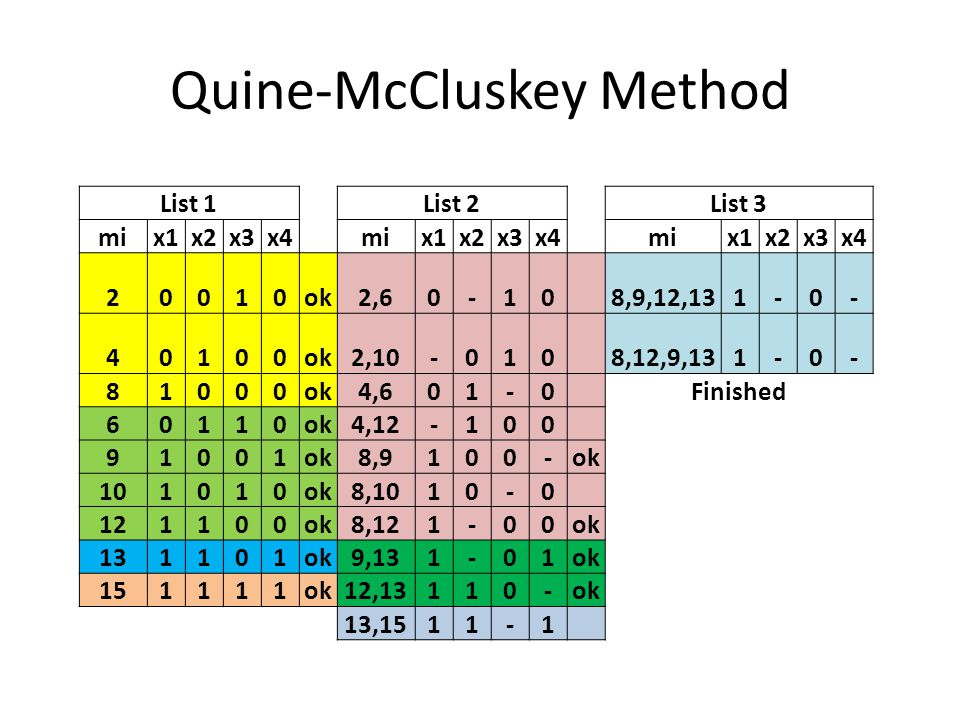
\includegraphics[scale=0.5]{images/QM.jpg}
		\caption{最小项表}
	\end{figure}
	
	由于Quine–McCluskey算法的描述比较清晰,按描述模拟即可。
	
	\lstinputlisting{sources/algo_part3.txt}	

\subsubsection{化简}
	化简分为两步:
	\begin{itemize}
		\item	若一个最小项只被一个质蕴涵包含,则该质蕴涵必须选
		\item	若剩余未被覆盖的最小项均被多个质蕴涵包含,则运用petrick算法进行化简
	\end{itemize}
\paragraph{基础化简\\}
	首先进行筛选,若一个最小项只被一个质蕴涵包含,则直接标记该质蕴涵为已选

	\lstinputlisting{sources/algo_part4.txt}	

\paragraph{进阶化简\\}
	若出现以下这种情况,基本的化简就无计可施了:

	\begin{figure}[h]
		\centering
		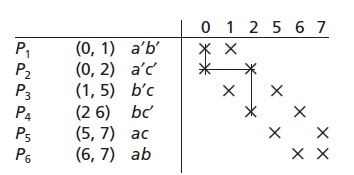
\includegraphics[scale=1]{images/petrick.jpg}
	\end{figure}

	即每个最小项都被至少两个质蕴涵覆盖。
	
	通用的算法是使用petrick化简,但是由于本题数据范围较小,可以直接对剩下的质蕴涵,直接穷举它是否被取,然后从所有方案中取选择质蕴涵最少的方案。
	
	这种方法的时间复杂度为$O(2 \land \mbox{剩余质蕴涵个数})$,由于剩余质蕴涵个数不会超过$2 ^ {n/2}$,因此时间复杂度不会超过$2 ^ {16} = 65536$,是完全可以接受的
	
	\lstinputlisting{sources/algo_part5.txt}	

\section{测试}

\subsection{正确性测试}
	首先,对于程序的正确性进行测试
	
	\paragraph{expr$\_$to$\_$truthtable\\}
		\lstinputlisting{sources/test_part0.txt}
	\paragraph{truthtable$\_$to$\_$expr\\}
		\lstinputlisting{sources/test_part1.txt}	
	\paragraph{cross$\_$validation\\}
		\lstinputlisting{sources/test_part2.txt}	
\subsection{健壮性测试}
	检测程序对于异常输入的处理	
	\paragraph{expr$\_$to$\_$truthtable\\}
		划分等价类:
		\begin{center}
			\begin{tabular}{cc}
				错误类型 & 抛出异常\\
				空串 & EmptyStringError\\
				非法字符 & InvalidCharError\\
				参数个数错误 & InvalidVariableError\\
				语法错误 & SyntaxError\\
				括号不匹配 & BracketMismatchingError\\
				正常输入 & No Error\\
		\end{tabular}				
		\end{center}

		\lstinputlisting{sources/test_part3.txt}
	\paragraph{truthtable$\_$to$\_$expr\\}
		划分等价类:
		\begin{center}
			\begin{tabular}{cc}
				错误类型 & 抛出异常\\
				空串 & EmptyStringError\\
				非法字符 & InvalidCharError\\
				参数个数$!=2^n$ & InvalidLengthError\\
				正常输入 & No Error\\
		\end{tabular}				
		\end{center}

		\lstinputlisting{sources/test_part4.txt}	
\subsection{效率测试}


\section{总结与体会}

这次project给我的帮助主要有两点: 学习了新的算法和认识到了测试的重要性。

完成这个Project大概花了我两个星期时间,其中确立思路与框架花了一天,写程序花了两天,剩下的时间都用于调试与测试数据。以前我对测试的重要性有所忽视,总认为反正程序很短,运用中可以出了问题再改。但是这次的工程量略微上升了一点,这种方法的弊病就出现了。对于一个表达式而言,需要考虑的corner case非常多。如果程序不能有一个很好的架构的话,很难考虑到所有情况,调试将会变得非常麻烦。因此,程序的合理组织比正确的写出程序更加重要。

而就这个project而言,它需要的两个函数expr$\_$to$\_$truthtable和truthtable$\_$to$\_$expr,我分别用了两个类ExpressionToChart和ChartToExpression来完成,而在ChartToExpression中,针对质蕴涵项这个概念被多次使用的情况,又另见了$implication$类来专门实现质蕴涵的相关操作。这样,这个project的架构就比较清晰,也比较利于调试了。

当然,这次project让我学习了Q-M算法和petrick化简,同时也复习了表达式求值这以经典算法。在实现上来说,表达式求值相对易于实现,因此expr$\_$to$\_$truthtable这个函数实现的较为轻松。而Q-M算法是我较为陌生的一种算法,较为繁琐。我在实现时也遇到了一些困难,但主要是由于我对于算法不太熟悉,思路不够清晰。经过几次的重构,这一部分才算完成。《孙子兵法》中说:“谋定而后动,知止而有得”。对于一个工程来说,要时刻保持思路的清晰,这比纯粹的垒代码重要的多。

很惭愧,就做了一点微小的工作。Linus Torvalds说过:“Talk is cheap, show me the code.”希望以这次的Mini$\_$Project作为起步,通过期末的Final$\_$Project,在实践中不断提示自己的工程能力。

\vspace{2cm}

\begin{figure}[h]
	\centering
		
\includegraphics[scale=0.8]{images/linus.png}
\end{figure}
\end{spacing}

%=================

\end{document}
